\section*{Exercício 1}

\begin{enumerate}
    \item[\textbf{a)}] É a variação do valor de saída provocada por uma variação da entrada, ambas em regime permanente.
    \item[\textbf{b)}] É a menor variação da entrada detectável por tal instrumento quando o valor inicial da entrada for diferente de zero.
    \item[\textbf{c)}] É o menor valor de entrada necessário para que o instrumento comece a apresentar uma indicação diferente de zero.
    \item[\textbf{d)}] É o comportamento de atraso na resposta de um instrumento que depende da direção da variação da entrada.
    \item[\textbf{e)}] Faixa de valores de entrada que pode ser percorrida após uma mudança de sentido de variação da entrada, sem provocar uma mudança observável no sinal de saída.
    \item[\textbf{f)}] Caracteriza o quanto a relação entre a entrada e a saída de um instrumento se aproxima de uma reta de referência.
    \item[\textbf{g)}] É a faixa de valores estáticos que o instrumento pode medir.
    \item[\textbf{h)}] É a diferença algébrica entre os valores extremos da faixa do instrumento.
    \item[\textbf{i)}] É a capacidade de um instrumento de fornecer o mesmo resultado quando uma mesma medição é repetida várias vezes sob condições idênticas.
    \item[\textbf{j)}] Grau de concordância entre resultados de medições do mesmo mensurando realizadas sob condições variadas de medição.
    \item[\textbf{k)}] Procura quantificar o período de tempo em que o instrumento fica livre de falhas.
    \item[\textbf{l)}] É o conjunto de operações que estabelece, sob condições especificadas, a relação entre os valores indicados por um instrumento de medição e os valores correspondentes realizados por um padrão de referência.
\end{enumerate}

\section*{Exercício 2}

\begin{enumerate}
    \item[\textbf{a)}] \textbf{Sensibilidade do sensor ($S$):}
    \[
    S = \frac{\Delta y}{\Delta x} = \frac{0{,}80 - 0{,}20}{10 - 0} = 0{,}06\text{ V/mm}
    \]

    \item[\textbf{b)}] \textbf{Equação da saída em função do deslocamento:}
    \[
    y(x) = 0{,}06x + 0{,}20 \quad [\text{onde } x \text{ está em mm e } y \text{ em V}]
    \]

    \item[\textbf{c)}] \textbf{Tensão de saída para $x = 35\text{ mm}$:}
    \[
    y(35) = 0{,}06(35) + 0{,}20 = 2{,}10 + 0{,}20 = 2{,}30\text{ V}
    \]

    \item[\textbf{d)}] \textbf{Justificativa da sensibilidade constante:}
    A taxa de variação $\frac{\Delta y}{\Delta x}$ entre todos os pontos consecutivos da tabela é rigorosamente constante e igual a $0{,}06\text{ V/mm}$, o que caracteriza uma resposta estática perfeitamente linear.

    \item[\textbf{e)}] \textbf{Deslocamento para $y = 2{,}45\text{ V}$:}
    \[
    2{,}45 = 0{,}06x + 0{,}20 \implies 0{,}06x = 2{,}25 \implies x = \frac{2{,}25}{0{,}06} = 37{,}5\text{ mm}
    \]
\end{enumerate}

\section*{Exercício 3}

Dada a relação:
\[
y(x) = 0{,}5 + 0{,}04x + 0{,}0008x^2 \quad \left[x \text{ (mm)}, \, y \text{ (V)}\right]
\]

\begin{enumerate}
    \item[\textbf{a)}] Sensibilidade estática (derivada):
    \[
    \frac{dy}{dx} = 0{,}04 + 2 \cdot 0{,}0008x = 0{,}04 + 0{,}0016x
    \]

    \item[\textbf{b)}] 
    \begin{itemize}
        \item Para $x = 10\text{ mm}$:
        \[
        y = 0{,}04 + 0{,}0016 \cdot 10 = 0{,}04 + 0{,}016 = 0{,}056
        \]
        \item Para $x = 40\text{ mm}$:
        \[
        y = 0{,}04 + 0{,}0016 \cdot 40 = 0{,}04 + 0{,}064 = 0{,}104
        \]
    \end{itemize}
\end{enumerate}

\section*{Exercício 4}

\begin{enumerate}
    \item[\textbf{a)}] \textbf{Tabela e Gráfico Comparativo:}
    
    \begin{table}[h!]
        \centering
        \begin{tabular}{cccc}
            \toprule
            $T$ ($^\circ\text{C}$) & $V_{\text{medido}}$ (V) & $V_{\text{ref}} = 0{,}10 + 0{,}049T$ (V) & Erro $e(T)$ (V) \\
            \midrule
            0   & 0{,}10 & 0{,}10 & 0{,}00 \\
            20  & 1{,}05 & 1{,}08 & $-0{,}03$ \\
            40  & 2{,}10 & 2{,}06 & $+0{,}04$ \\
            60  & 3{,}02 & 3{,}04 & $-0{,}02$ \\
            80  & 4{,}08 & 4{,}02 & $+0{,}06$ \\
            100 & 5{,}00 & 5{,}00 & 0{,}00 \\
            \bottomrule
        \end{tabular}
    \end{table}

    \item[\textbf{b)}] \textbf{Erro ponto a ponto:}
    \[
    e(T) = V_{\text{medido}}(T) - V_{\text{ref}}(T)
    \]
    O erro máximo absoluto é $e_{\max} = 0{,}06\text{ V}$ (em $T = 80^\circ\text{C}$).

    \item[\textbf{c)}] \textbf{Linearidade Estática:}
    \[
    \text{FSO} = V_{\max} - V_{\min} = 5{,}00 - 0{,}10 = 4{,}90\text{ V}
    \]
    \[
    \text{NL}_{\%} = \left(\frac{e_{\max}}{\text{FSO}}\right) \times 100 = \left(\frac{0{,}06}{4{,}90}\right) \times 100 \approx 1{,}22\%
    \]
\end{enumerate}
\section*{Exercício 5}

\begin{enumerate}
    \item[\textbf{a)}] V
    \item[\textbf{b)}] V
    \item[\textbf{c)}] F
    \item[\textbf{d)}] V
    \item[\textbf{e)}] V
    \item[\textbf{f)}] F

\end{enumerate}

\section*{Exercício 6}

\begin{enumerate}
    \item[\textbf{a)}] $0{,}5\text{ kPa}$
    \item[\textbf{b)}] $2\text{ kPa}$
    \item[\textbf{c)}] Não, pois ele precisa de $2\text{ kPa}$ para começar a detectar a partir do repouso.
    \item[\textbf{d)}] Também não, pois o sensor só detecta variações de $0{,}5\text{ kPa}$ após deixar o repouso.
    \item[\textbf{e)}] Resolução é o valor necessário para o sensor começar a perceber a característica da grandeza física a ser medida. Já o limiar determina o quão sensível o sensor é à variação da característica física a ser medida.
\end{enumerate}

\section*{Exercício 7}

\begin{enumerate}
    \item[\textbf{a)}] 
    \begin{align*}
    0 &\to 0{,}10 - 0{,}10 = 0 \\
    20 &\to 1{,}05 - 1{,}00 = 0{,}05 \\
    40 &\to 2{,}02 - 1{,}92 = 0{,}10 \\
    60 &\to 3{,}08 - 2{,}88 = 0{,}20 \\
    80 &\to 4{,}05 - 3{,}91 = 0{,}14 \\
    100 &\to 5{,}00 - 5{,}00 = 0
    \end{align*}

    \item[\textbf{b)}] 
    \[
    y_{\min} = 0{,}10, \quad y_{\max} = 5{,}00, \quad e_{h,\max} = 0{,}2
    \]
    \[
    e_{h\%} = \frac{e_{h,\max}}{y_{\max} - y_{\min}} = \frac{0{,}2}{5{,}00 - 0{,}10} = 0{,}04082 \quad (\approx 4{,}08\%)
    \]
\end{enumerate}

\section*{Exercício 8}

\begin{enumerate}
    \item[\textbf{a)}] V \quad \textbf{e)} V
    \item[\textbf{b)}] F \quad \textbf{f)} F
    \item[\textbf{c)}] F \quad \textbf{g)} F
    \item[\textbf{d)}] --- \quad \textbf{h)} F
    \item[\textbf{i)}] V
\end{enumerate}

\section*{Exercício 9}

Valores médios:
\begin{itemize}
    \item Operador A: $0{,}02$
    \item Operador B: $10{,}31 - 10{,}28 = 0{,}03$
    \item Operador C: $9{,}82 - 9{,}80 = 0{,}02$
\end{itemize}
Sendo $F_s = 10$:
\[
\text{Rep}_A\% = \left(\frac{0{,}02}{10}\right) \times 100 = 0{,}2\%
\]
\[
\text{Rep}_B\% = \left(\frac{0{,}03}{10}\right) \times 100 = 0{,}3\%
\]
\[
\text{Rep}_C\% = \left(\frac{0{,}02}{10}\right) \times 100 = 0{,}2\%
\]
\textit{Então os valores são extremamente baixos, o que representa excelente repetibilidade.}

\section*{Exercício 10}

É uma expressão matemática que descreve a relação entre a entrada e a saída de um instrumento de medição. Simplifica a análise de sistemas dinâmicos, facilita a previsão de resposta, avalia o desempenho e a estabilidade do sistema em questão.

\section*{Exercício 11}

Descreve como um instrumento responde a sinais senoidais de diferentes frequências.

\section*{Exercício 12}

\begin{itemize}
    \item \textbf{Sistemas de ordem zero:} São uma reta constante em um único valor.
    \item \textbf{Sistemas de primeira ordem:} São caracterizados por uma curva exponencial onde podemos analisar a constante de tempo (que indica quanto tempo o sistema leva para atingir o valor final) e o ganho estático (que representa o valor final da saída em relação à entrada).
    \item \textbf{Sistemas de segunda ordem:} São caracterizados por uma curva que depende de suas características dinâmicas, onde podemos analisar o ganho (relação entre o valor final e o valor de entrada), a frequência natural (define a velocidade de resposta do sistema) e o fator de amortecimento (determina o grau de amortecimento do sistema).
\end{itemize}

\section*{Exercício 13}

\begin{enumerate}
    \item[\textbf{a)}] Sistema de segunda ordem.
    \item[\textbf{b)}] Sistema de primeira ordem.
\end{enumerate}

\section*{Exercício 14}

Circuito RC:
\[
\tau = R \cdot C \implies 2 = R \cdot C
\]
Convencionando $C = 100\,\mu\text{F}$:
\[
R = \frac{2}{100 \cdot 10^{-6}} = 20\text{ k}\Omega
\]

\section*{Exercício 15 \& Dedução do Amortecimento}

Dos valores do gráfico temos:
\[
M_p = 1{,}6, \quad t_{5\%} = 0{,}07 \quad \left(\text{onde } 0{,}07 = \frac{3}{\zeta \omega_n}\right)
\]

Dedução de $\zeta$ (ou $L$):
\[
1{,}6 = e^{\frac{-\pi \zeta}{\sqrt{1 - \zeta^2}}}
\]
\[
\ln(1{,}6) = \frac{-\pi \zeta}{\sqrt{1 - \zeta^2}}
\]
\[
\left(\ln 1{,}6\right)^2 \cdot (1 - \zeta^2) = (-\pi \zeta)^2 = \pi^2 \zeta^2
\]
\[
(\ln 1{,}6)^2 - \zeta^2 (\ln 1{,}6)^2 = \pi^2 \zeta^2
\]
\[
(\ln 1{,}6)^2 = \zeta^2 \left[ (\ln 1{,}6)^2 + \pi^2 \right]
\]
\[
\zeta = \sqrt{\frac{(\ln 1{,}6)^2}{(\ln 1{,}6)^2 + \pi^2}} \implies \zeta = 0{,}16
\]

Cálculo da frequência natural ($\omega_n$):
\[
\omega_n = \frac{3}{\zeta \cdot 0{,}07} = \frac{3}{0{,}16 \cdot 0{,}07} = 267{,}86 \text{ rad/s}
\]

Função de Transferência $H(s)$:
\[
H(s) = \frac{(267{,}86)^2}{s^2 + 2 \cdot 0{,}16 \cdot 267{,}86 \cdot s + 267{,}86^2} = \frac{71746{,}98}{s^2 + 80{,}36 s + 71746{,}98}
\]

\section*{Exercício 16}

\[
t_{5\%} = \frac{3}{0{,}16 \cdot 267{,}86} = 0{,}07\text{ s}
\]
\textit{É o tempo que um instrumento leva para atingir e se manter dentro de uma estreita faixa em torno de seu valor em regime permanente, após ter sido excitado por uma entrada degrau.}

\section*{Tempos de Resposta e Sobressinal}

\subsection*{Tempo de Subida ($t_r$)}
\[
t_r = \frac{2{,}16 \cdot 0{,}16 + 0{,}6}{267{,}87} = 3{,}23 \times 10^{-3} \text{ s}
\]
\textit{É o tempo gasto para que a resposta passe de 10\% para 90\% de seu valor.}

\subsection*{Tempo de Pico ($t_p$)}
\[
t_p = \frac{\pi}{267{,}87 \cdot \sqrt{1 - 0{,}16^2}} = 0{,}011885\text{ s}
\]
\textit{É o tempo necessário para a resposta atingir o primeiro pico do sobressinal.}

\subsection*{Sobressinal Máximo ($M_p$)}
\[
M_p = e^{\frac{-\pi \cdot 0{,}16}{\sqrt{1 - 0{,}16^2}}} = 0{,}600
\]
\textit{É a diferença entre o valor do primeiro pico da resposta e o valor final da resposta.}

\section*{Exercício 17}

Sendo a função dada por:
\[
V(F) = 0{,}049 F + \cancelto{0}{0{,}05381}
\]
\[
V(s) = 0{,}049 F(s)
\]
\[
\frac{V(s)}{F(s)} = 0{,}049
\]

Para a resposta em frequência:
\[
|G(j\omega)| = 0{,}04911 \approx -26{,}17 \text{ dB}
\]
\[
\text{Fase } \Theta(\omega) = 0^\circ
\]

\vspace{0.5cm}

\noindent $F_{\min} = 0\text{ N} \implies V_{\min} = 0{,}10\text{ V}$ \\
$F_{\max} = 100\text{ N} \implies V_{\max} = 5{,}00\text{ V}$

\[
K = \frac{\Delta V}{\Delta F} = \frac{5{,}00 - 0{,}10}{100 - 0} = \frac{4{,}90}{100} = 0{,}049
\]

\vspace{0.5cm}

\noindent Considerado modelo dinâmico de 1ª ordem:
\[
G(s) = \frac{K}{\tau s + 1} = \frac{0{,}049}{s + 1}
\]
Com $\tau = 1$ (valor genérico).


\begin{lstlisting}

import matplotlib.pyplot as plt
from scipy import signal

# G(s) = 0.049 / (s + 1)
sys = signal.TransferFunction([0.049], [1.0, 1])

t, y = signal.step(sys)
w, mag, phase = signal.bode(sys)

plt.figure(figsize=(10, 10))
plt.subplot(3, 1, 1)
plt.plot(t, y)
plt.title('Resposta ao Degrau')

plt.subplot(3, 1, 2)
plt.semilogx(w, mag)
plt.title('Bode (Magnitude)')

plt.subplot(3, 1, 3)
plt.semilogx(w, phase)
plt.title('Bode (Phase)')
\end{lstlisting}
\begin{figure}[h!]
    \centering
    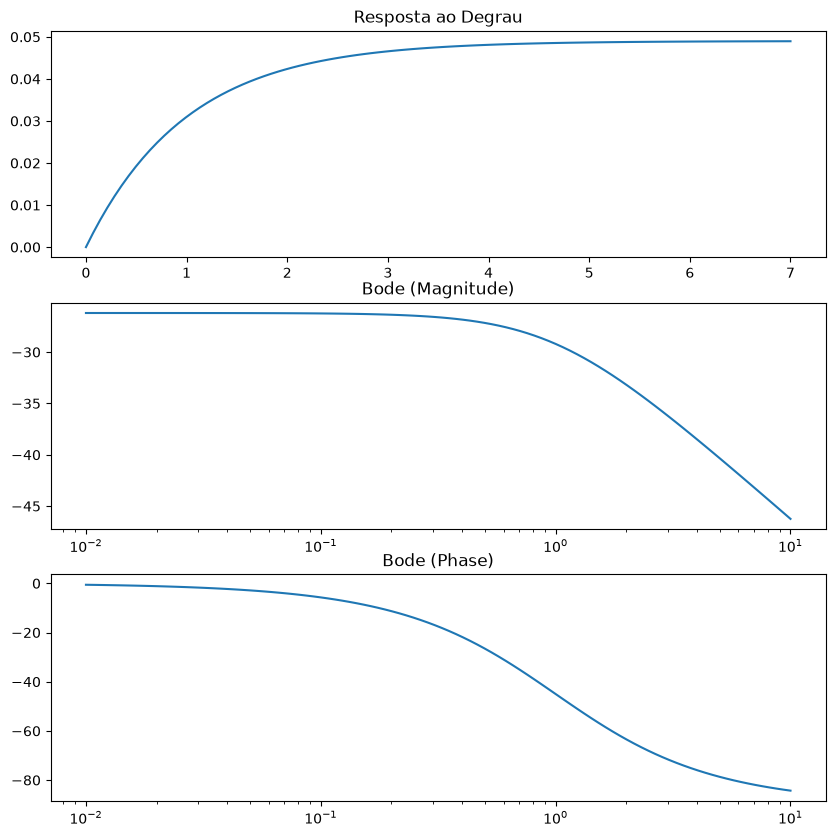
\includegraphics[width=0.8\textwidth]{image.png}
    \caption{plotagem das respostas do sistema de 1ª ordem.}
    \label{fig:minha_imagem}
\end{figure}